% !TeX spellcheck = en_US

\chapter{A programming model for OSRA}
\label{chap: Progamming model}

\section{Introduction}
In the previous chapters we have seen the model-driven software development approach that was centered on component-based techniques. Dijkstra's principle of separation of concerns was one of the cornerstone principles which was part of the software reference architecture and the component model proposed \cite{CompBasedProcess,EvoRAVCodeAr}. According to it, the user design space should be limited to the internals of the components, where only strictly sequential code can be used and the extra non-functional requirements are declaratively specified in the form of annotations on the component provided interfaces. This is already explained in detail in Step 7 (Specification of non-functional attributes) in \cref{chap: Software development process}. 

As discussed in the previous chapters, the reference software architecture is made up of a component model, a computational model, a programming model and a conforming execution platform. It is also clear that the component model should be statically bound to a computational model to formally define the computational entities and the rules which govern their usage.

The realization of extra functional properties or more precisely, the generation of the complete infrastructure code can be done in two steps:
\begin{itemize}
\item Automated generation of the non-functional code i.e., the code for handling concurrency and interaction requirements for communication between components and the skeletons for the components themselves
\item Automated generation of containers for components and the connectors between components 
\end{itemize}

A code generator needs to be developed for this purpose and the next few chapters would be concerned about realizing the above mentioned steps. As a result, the third-party software supplier can solely concentrate on implementing the functional code of the components. This is in line with the principle of separation of concerns, which is of very high interest.

The ASSERT project (Automated proof-based System and Software Engineering for Real-Time systems) aimed at the definition of a MDE design process for the development of on-board software for satellites, cenetered on the priciples of correctness-by-construction and separation of concerns \cite{PhdThesis}. The cornerstone of the project is the adoption of an infrastrcuture called the Ravenscar Computational Model (RCM) \cite{PhdThesis}. This modeling infrastructure which was developed at the University of Padua \cite{ScheduAnaly} included a graphical modeling language and its editor, a model validator and a set of model transformations to feed the model-based schedulability analysis and code generation \cite{ScheduAnaly}. It is important to note that the ASSERT project lacked an explicit notion of a component model but incporporated a computational model, a programming model and a conforming execution platform \cite{PhdThesis}. Certain Ada Ravenscar Profile compliant code archetypes were developed to complete the formulation of the programming model and these archetypes adhered to the vision of principle of separation of concerns and amenable to code generation \cite{CharEvoRAVCodeAr}. The Ada Ravenscar Profile basically does not allow any Ada language constructs that are exposed to unbounded execution-time and non-determinism \cite{RAVCodeAr}. The code archetypes used Ada run-time and hence could fit the needs of typical embedded systems which were resource-constrained \cite{RAVCodeAr}.   

In the following Artemis JU CHESS project, an initiative from ESA in parallel to the development of the SCM \cite{CompBasedProcess, PhdThesis}, a computational model named as Ravenscar Computational Model (RP in the following text) was chosen as the computational model \cite{ScheduAnaly}. RP directly emanated from the Ada Ravenscar Profile in language-neutral terms \cite{CharEvoRAVCodeAr,EvoRAVCodeAr}. The code archetypes from the ASSERT project were revised and extended in the CHESS project and they as well targeted the Ada Ravenscar Profile, for the additional reason that the reduced tasking model used in the Ada Ravenscar Profile matched the semantic assumptions and communication model of real-time theory, the response-time analysis in particular \cite{CharEvoRAVCodeAr}. The code archetypes developed in the CHESS project \cite{EvoRAVCodeAr} are taken as reference for developing a programming model in this chapter. The code archetypes discussed in this Master thesis, however, target the Tasking framework which is the chosen computational model for this Master thesis. The reasons for choosing Tasking framework as a computational model is already explained at the end of the previous chapter. The code archetypes discussed in this chapter are first steps towards generation of the complete infrastructural code. 

\section{Structure of the code archetypes}
The code archetypes discussed in this Master thesis strive to attain as much separation as possible between the functional and extra-functional/non-functional concerns. At the implementation level, functional/algorithmic code of a component is separated from the code that manages the realization of the extra-functional requirements like tasking, synchronization and different time-related aspects.

The library of sequential code, which may have as many cohesive operations as the software supplier wishes to include in a single executing component, is included in a closed structure such as a component implementation. The mapping of this structure to the actual design entity of the infrastructural code is not of concern in handled in the next chapter. The sequential code in this structure is executed by a distinct flow of control of the system. The dedicated flow of control can be an active task, together with other tasking primitives from the Tasking framework (if the desired concurrency kind is \texttt{asynchronous}). Or, it can be a simple synchronous method/operation invocation, which uses the flow of control of the component requesting the service from outside (if the desired concurrency kind is \texttt{synchronous}). This leads to a combined effect that the component internals are completely hidden from outside environment, and the provided services invoked by the external clients are executed with the desired interaction semantics.

As multiple clients may independently require a range of services to be executed by one of the two desired flow of controls i.e. \texttt{synchronous} or \texttt{asynchronous}, it is necessary to safeguard these execution requests from mixing up. Safeguarding of execution requests in case of synchronous service requests is implicit as these requests would have been raised in the respective flow of control of the component asking for the service, but the safeguarding of execution requests in case of asynchronous requests needs to be explicitly handled and the way to achieve this is explained in the next parts of this section.

Service requests can often lead to valid/invalid data that need to be sent back safely to the components which made the requests. The service requester also need to be informed about any exceptions that might arise due to any unexpected situations during the servicing of the requests. The mechanisms and semantics necessary for realizing these requirements are also explained in the next parts of this section. 

\subsection{Synchronous release patterns}
The archetypes for a synchronous release pattern are quite straight forward. When a request for a service is made with the desired concurrency kind specified as \texttt{synchronous}, the request is handled straight-away as a normal function/operation call in the flow of control of the service requester as shown in \cref{fig: Synchronous call}. The results (if any) from the service requests, and exceptions (if any) during the course of handling the service requests are returned back to the service requester using the same flow of control as shown in \cref{fig: Synchronous call}.

\begin{figure}[h]
	\centering
	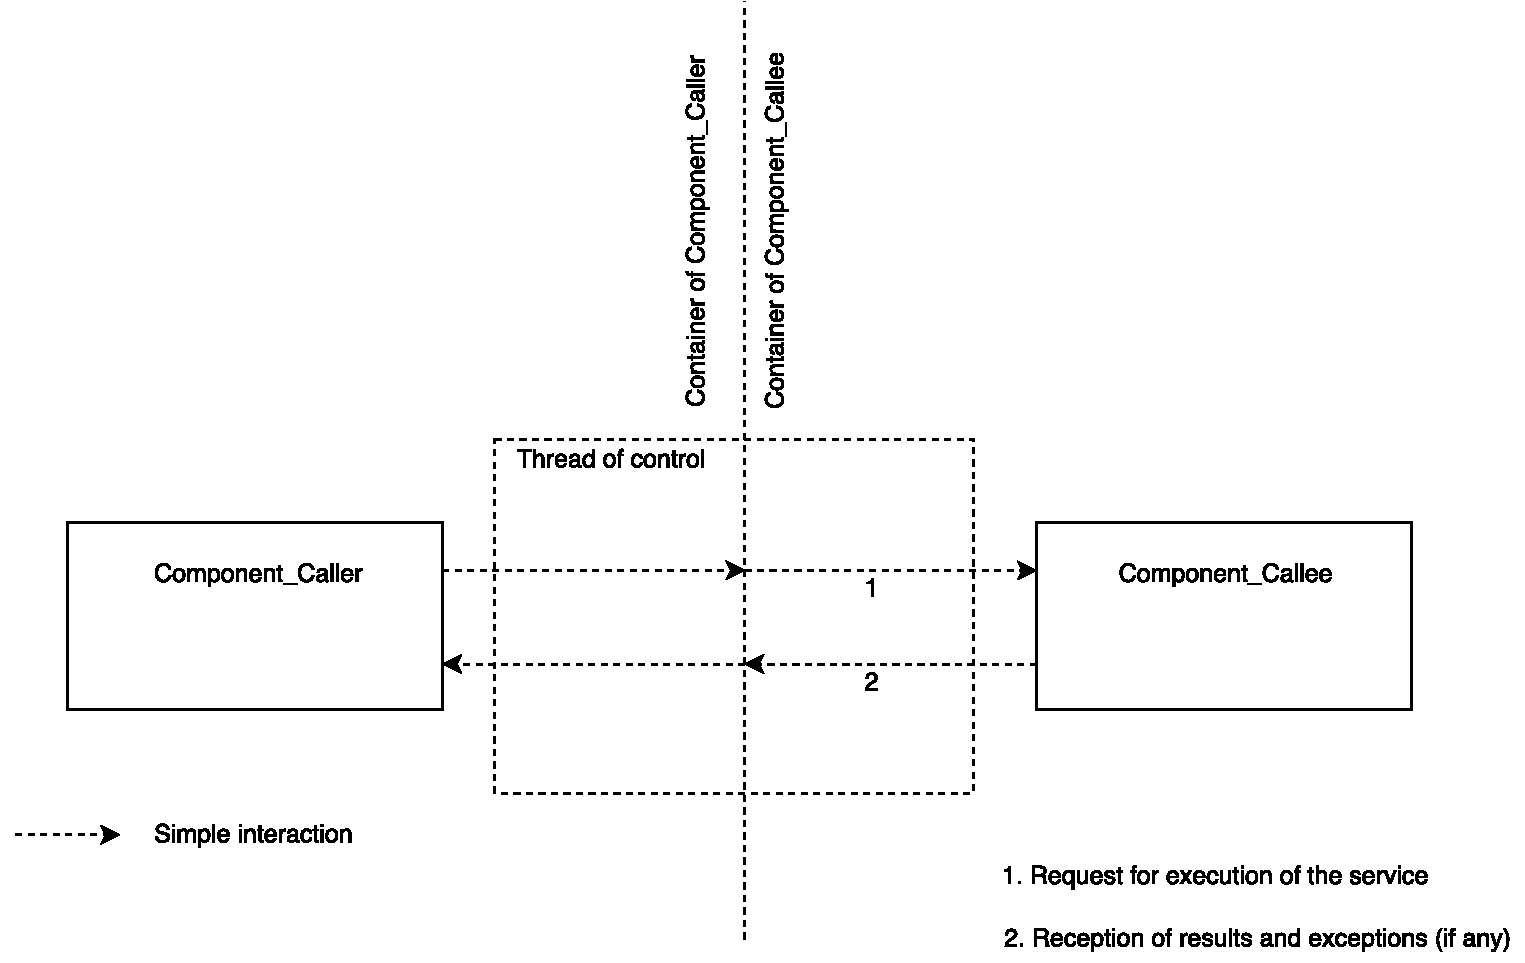
\includegraphics[width=0.8\textwidth]{Synchronous.pdf}
	\caption{Synchronous release pattern}
	\label{fig: Synchronous}
\end{figure}

\subsubsection{\textbf{Protected}}
When the non-functional property set on the service in the provided interface side of the component offering the service is \texttt{Protected}, it is necessary for the container that wraps around the component to safeguard this non-functional property. As the container is the entity that promotes the provided interface of the component, it intercepts the function/operation call from outside and provides exclusive access to the service implemented by the component. Semaphores provided by the Tasking framework is used for this purpose.

\subsubsection{\textbf{Unprotected}}
When the non-functional property set on the service in the provided interface side of the component offering the service is \texttt{Unprotected}, the semantics of handling the service request is essentially the same as the way the protected operations are handled, except for the fact that obtaining and releasing of the semaphore for the operation is not anymore needed.

\subsection{Asynchronous release patterns}
The archetypes for asynchronous release patterns are quite complicated when compared to archetypes for synchronous release patterns. As the requests cannot be anymore handled in the flow of control of the service requester in case of asynchronous release pattern, tasks from Tasking framework along with other tasking primitives, which are independent threads of execution can be activated to cater to these requests on the provided interface side. 

The asynchronous service request is initially intercepted at the required interface port subsumed by the container of the component which makes the request. Here the data (if any), associated with the request is packaged and the packaged data is forwarded to the provided interface port, which is promoted by the container of the component handling the request. Along with the data associated with the service request, it is also important that the required interface port packages information about how to send back the results and exceptions (if any) to the service requester.

In case of asynchronous service requests, if the service request leads to an exception being raised at the service provider end, it is the responsibility of the service requester to cope up with the exception and it is of no interest in this Master thesis. This Master thesis, however, explains how the information about the raised exception needs to be delivered to the service requester. 

Each thread of control, having its own structure as explained above, is responsible for only one operation in the provided interface side of the component. As the release patterns for requests are already decided statically and as these release patterns are not expected to change at run-time, the number of threads of control that will be necessary to handle the service requests will be known at compile-time.

This is very similar to the way asynchronous release patterns are handled in the code archetypes listed in \cite{CharEvoRAVCodeAr,EvoRAVCodeAr} except for the fact that they do not consider service requests which might result in results or exceptions that need to be sent back to the service requester \cite{CharEvoRAVCodeAr}. 

\subsubsection{\textbf{Sporadic}}
When the non-functional property set for the handling of the service on the provided interface side of the component offering the service is \texttt{Sporadic}, it is the responsibility of the container, of the component providing the service, to safeguard this property. The sporadic property requires that two subsequent requests for the service needs to always be separated by no less but possibly more than a minimum guaranteed time span, known as the MIAT (Minimum Inter-Arrival Time) \cite{SpecMetamodel,CompBasedProcess}. The container makes use of tasking primitives such as a task channel, task event and a task from the Tasking framework for this purpose.

The general structure of the thread of control on the service provider end, necessary to handle sporadic service requests consists of a task with two synchronized task inputs, attached to the task as shown in \cref{fig: Asynchronous sporadic}. The task inputs are not marked as final. One of the task inputs is associated with a task event, with absolute timing (fixed task wake-up times) and the other task input is associated with a normal task channel. The task event is configured to wake up the task periodically after every MIAT interval. The task input associated with a normal task channel is configured so that the task input is activated as soon as a push is made against its associated task channel. This task then is instantiated in the container of the service provider component.   

When a provided interface port, promoted by the container of the component handling the request, receives a sporadic service release request, it intercepts the request and pushes the packaged data against the channel associated with the task. 

Because the task inputs are not marked as final, the task is activated only after both its task inputs are activated. When activated, the functions of the task will then be to:
 
\begin{description}
\item [Step 1] Unpack the packaged data
\item [Step 2] Acquire the semaphore provided by the Tasking framework associated with the service
\item [Step 3] Execute the desired service
\item [Step 4] Reset the task event attached to the task
\item [Step 5] Release the semaphore acquired 
\item [Step 6] Return the results and the exceptions associated with the service request back to the service requester making use of the information of the service requester packaged by the required interface port 
\end{description}

In this way, the non-functional properties associated with an asynchronous sporadic release pattern can be preserved at run-time.

\begin{figure}[h]
	\centering
	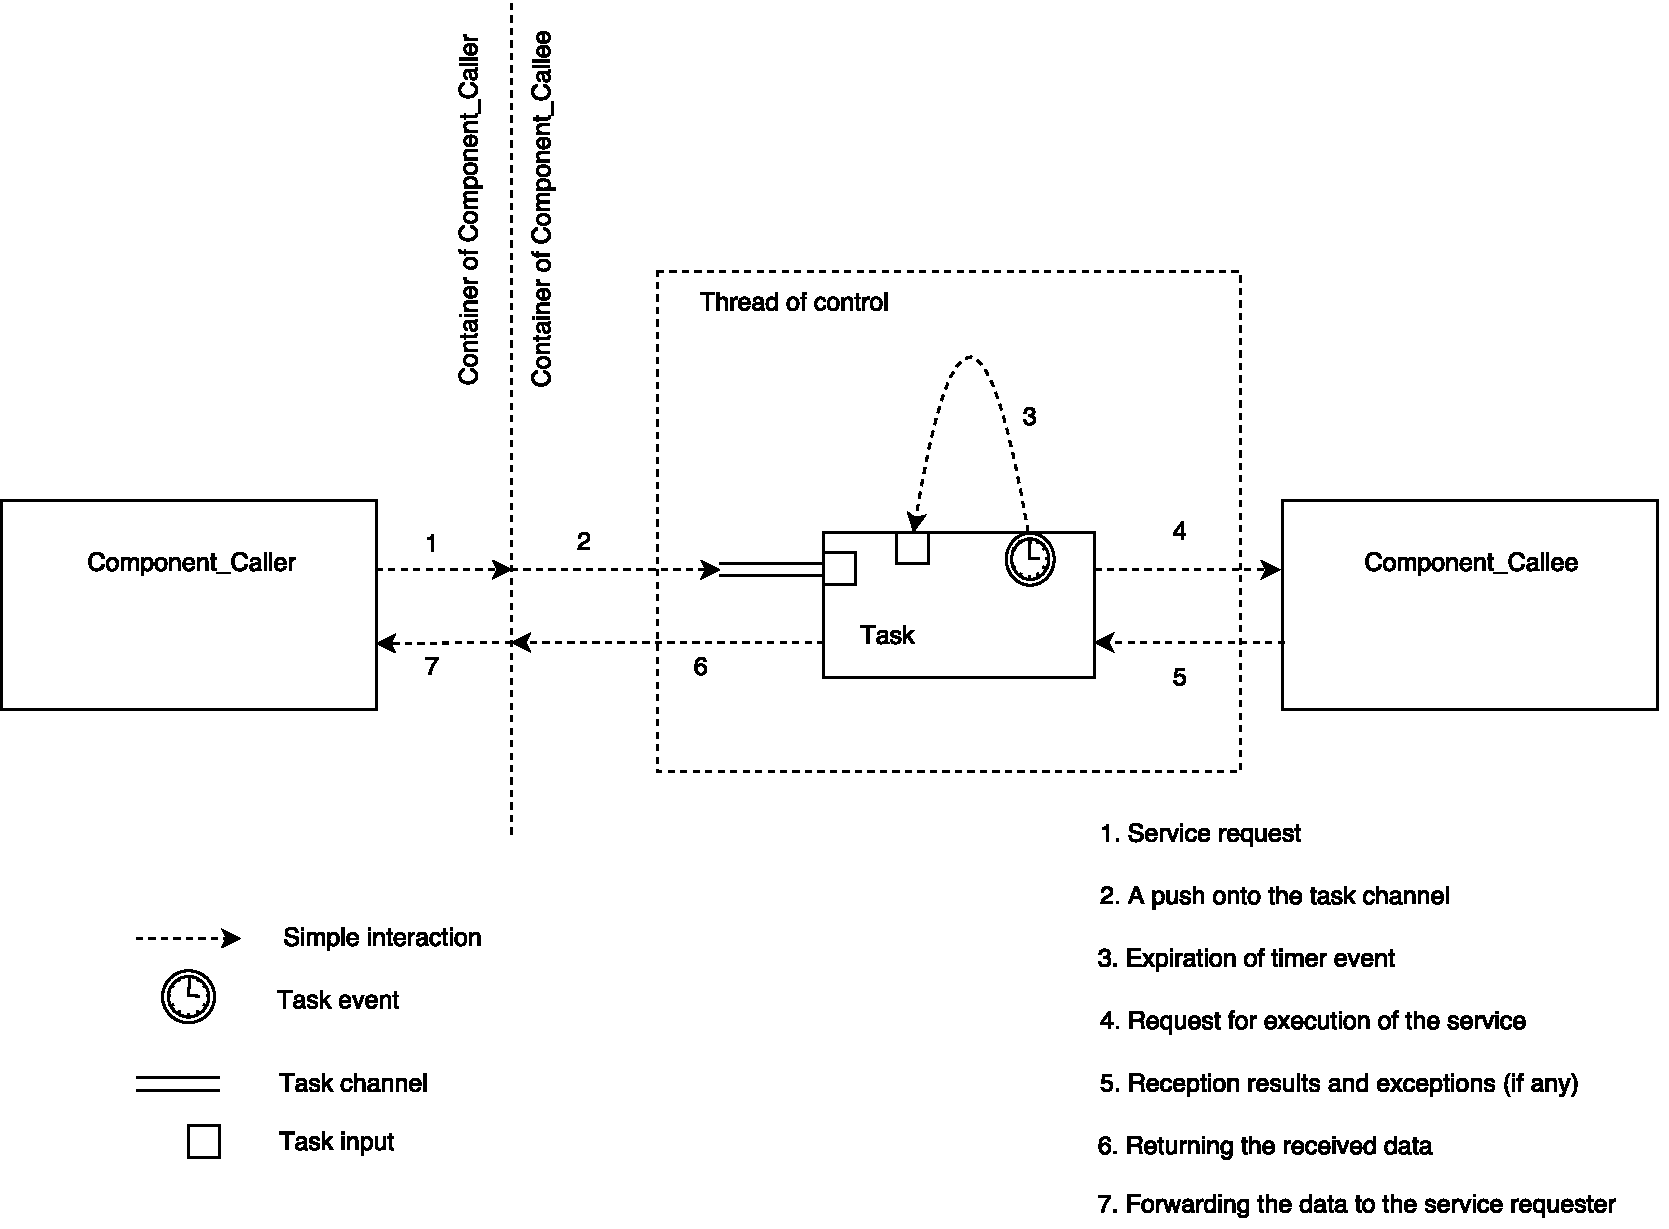
\includegraphics[width=0.8\textwidth]{AsynchronousSporadicOperation.pdf}
	\caption{Thread of control for asynchronous sporadic release pattern}
	\label{fig: Asynchronous sporadic}
\end{figure}

\subsubsection{\textbf{Protected}}
When the non-functional property set for the handling of the service on the provided interface side of the component offering the service is \texttt{Protected}, it is the responsibility of the container, of the component providing the service, to safeguard this property. The container makes use of tasking primitives such as a task channel and a task from the Tasking framework for this purpose. 

The general structure of the thread of control on the service provider end, necessary to handle this kind of service requests, is a task with one task input attached to the task as shown in \cref{fig: Asynchronous protected}. The task input is configured so that the task input is activated as soon as a push is made against its associated task channel.  

When a provided interface port, promoted by the container of the component handling the request, receives a service release request of this kind, it intercepts the request and pushes the packaged data against the channel associated with the task. The task is then activated and the functions of the task will then be to:

\begin{description}
\item [Step 1] Unpack the packaged data
\item [Step 2] Acquire the semaphore provided by the Tasking framework associated with the service
\item [Step 3] Execute the desired service
\item [Step 4] Release the semaphore acquired 
\item [Step 5] Return the results and the exceptions associated with the service request back to the service requester making use of the information of the service requester packaged by the required interface port 
\end{description}

In this way, the non-functional properties associated with an asynchronous protected release pattern can be preserved at run-time.

\begin{figure}[h]
	\centering
	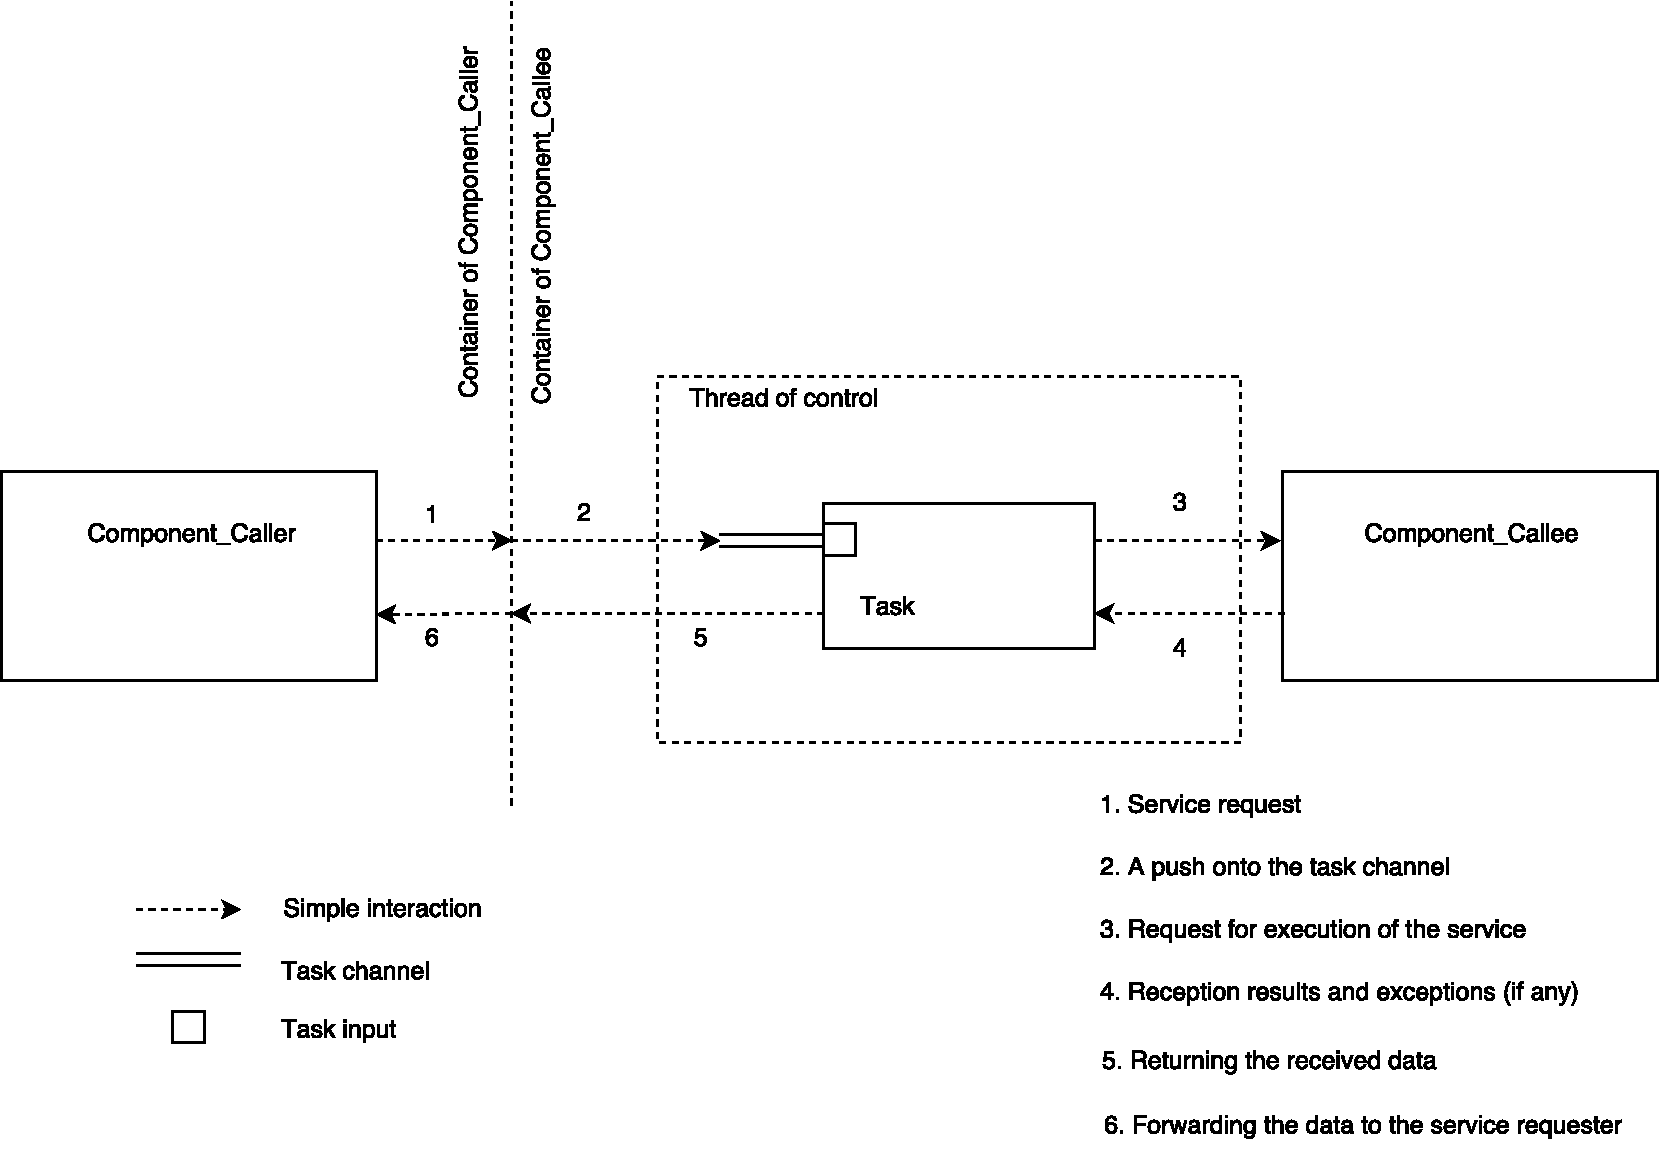
\includegraphics[width=0.8\textwidth]{AsynchronousProtectedOperation.pdf}
	\caption{Thread of control for asynchronous protected release pattern}
	\label{fig: Asynchronous protected}
\end{figure}

\subsubsection{\textbf{Bursty}}
When the non-functional property set for the handling of the service on the provided interface side of the component offering the service is \texttt{Bursty}, it is the responsibility of the container, of the component providing the service, to safeguard this property. The bursty property requires that a service can be activated at most a given number of times in a given interval called the bound interval \cite{SpecMetamodel,CompBasedProcess}.

The general structure of the thread of control on the service provider end, necessary to handle this kind of service requests, is a task with two non-synchronized task inputs attached to it as shown in \cref{fig: Asynchronous bursty}. The task inputs are marked as final. One of the task inputs is associated with a task event, with absolute timing (fixed task wake-up times) and the other task input is associated with a normal task channel. The task event is configured to wake up the task periodically after every bound interval. The task input associated with a normal task channel is marked as \texttt{final} indicating that the task input is activated as soon as a push is made against its associated task channel. The task also has an internal counting semaphore provided by the Tasking framework in order to keep a count of the number of service requests handled within the bound interval.

When a provided interface port, promoted by the container of the component handling the request, receives a service release request with bursty nature, it intercepts the request and pushes the packaged data against the channel associated with the task.
  
Because the task inputs are marked as final, the task is activated if any one of its task inputs are activated. When activated, the functions of the task will then be to:

\begin{description}
\item [Step 1] Check the activated input. If the activated input is the one that is attached to a task event, then replenish the counting semaphore, restart the attached task event and go to step 8. 
\item [Step 2] Unpack the packaged data
\item [Step 3] Acquire the counting semaphore local to the task which is used to enforce the max. number of activations within a bound interval
\item [Step 4] Acquire the semaphore provided by the Tasking framework associated with the service
\item [Step 5] Execute the desired service
\item [Step 6] Release the semaphore associated with the service 
\item [Step 7]Return the results and the exceptions associated with the service request back to the service requester making use of the information of the service requester packaged by the required interface port 
\end{description}

In this way, the non-functional properties associated with an asynchronous bursty release pattern can be preserved at run-time. It is important to note that the code archetypes which were developed for the CHESS project do not mention the scheme to handle this kind of release pattern \cite{CharEvoRAVCodeAr,EvoRAVCodeAr}.

\begin{figure}[h]
	\centering
	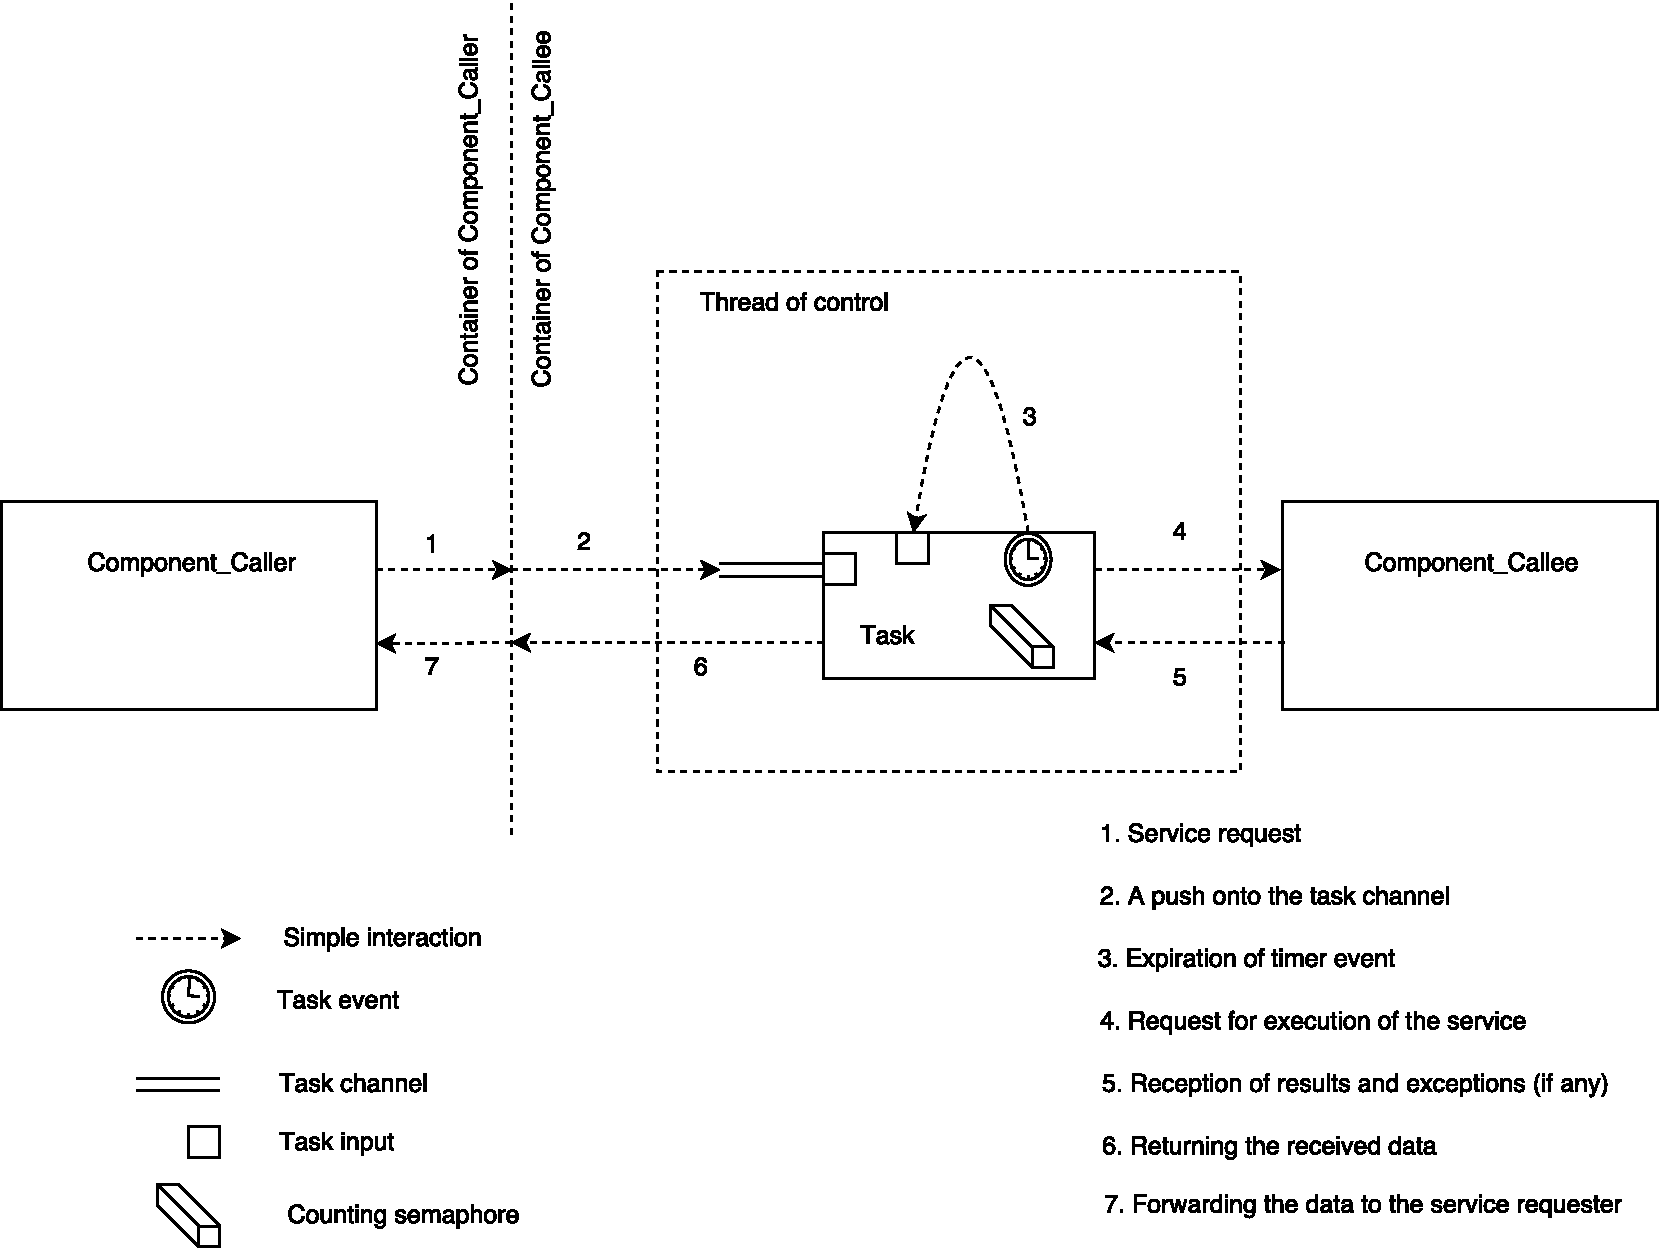
\includegraphics[width=0.8\textwidth]{AsynchronousBurstyOperation.pdf}
	\caption{Thread of control for asynchronous bursty release pattern}
	\label{fig: Asynchronous bursty}
\end{figure}

\subsubsection{\textbf{Cyclic}} 
When the non-functional property set for a service on the provided interface side of the component is \texttt{Cyclic}, it is the responsibility of the container of the component, to safeguard this property. Cyclic property requires that the associated service be activated periodically and with a non-zero initial offset \cite{SpecMetamodel,CompBasedProcess}. 

The general structure of the thread of control, necessary to handle this kind of non-functional property is a task with a task event, provided by the Tasking framework, attached to it as shown in \cref{fig: Asynchronous cyclic}. The task event is configured to wake up the task periodically, with absolute timing (fixed task wake-up times). The task event can also be configured to wake up the associated task for the very first time with an initial offset.

When a provided interface port, promoted by the container of the component has a service which needs to be activated periodically, the task is activated and it performs the following functions:

\begin{description}
\item [Step 1] Acquire the semaphore provided by the Tasking framework associated with the service
\item [Step 2] Execute the desired service
\item [Step 3] Release the semaphore acquired 
\end{description}    

The service with a cyclic nature cannot be requested from an external component \cite{SpecMetamodel}. The services also need to be parameterless and cannot send out results or throw exceptions \cite{SpecMetamodel}. 

In this way, the non-functional properties associated with an asynchronous cyclic release pattern can be preserved at run-time. 

\begin{figure}[h]
	\centering
	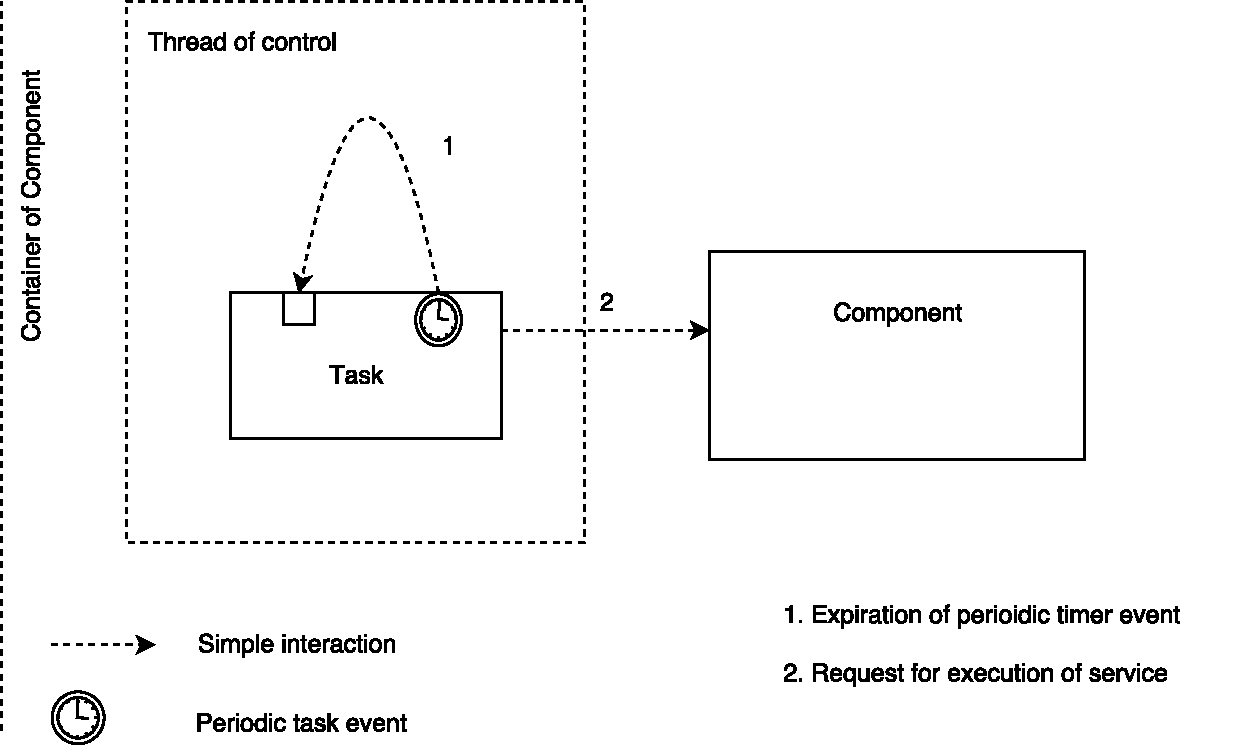
\includegraphics[width=0.8\textwidth]{AsynchronousCyclicOperation.pdf}
	\caption{Thread of control for asynchronous cyclic release pattern}
	\label{fig: Asynchronous cyclic}
\end{figure}  

   



 


 
